\chapter{Análisis y Diseño}
\label{chap:analisis_diseño}

\lettrine{E}{n} este capítulo se expone brevemente el análisis de requisitos que se ha realizado, así como ya más en profundidad las decisiones tomadas durante el diseño.

\section{Requisitos Hardware}
\label{sec:requisitos_hardware}
En esta sección se analizan los requisitos del proyecto, que han sido divididos en tres secciones en lugar de las tradicionales dos para mayor claridad, ya que el aspecto físico, así como las dimensiones del mismo son un aspecto muy importante a considerar.

\subsection{Requisitos Físicos}
Estos requisitos son de los más importantes debido a que modifican la estructura y limitaciones físicas del proyecto, conteniendo requisitos tanto funcionales como no funcionales, por lo que está en una sección a parte.

Primeramente conviene recordar que este trabajo se lleva a cabo durante la pandemia causada por el COVID-19, por lo que la movilidad es reducida y el teletrabajo desde el domicilio la regla. Bajo estas circunstancias se comienza a realizar un diseño que satisfaga los siguientes requisitos:
\begin{itemize}
    \item El cluster debe ser \textbf{pequeño} y \textbf{manejable}: Debido a que el trabajo se realiza desde casa, éste no puede ser muy extenso, ya que el espacio es muy limitado, por lo que se deben descartar estructuras donde los nodos quedan ``libres'' y ``desperdigados'' encima de una grande mesa.
    \item El cluster debe ser \textbf{visualmente agradable} y \textbf{comprensible}: Debido a que va a ser visto por personas con (posiblemente) escasa formación en \acrshort{hpc}, el cluster ha de tener partes fácilmente identificables, lo más aisladas y señalables posible, y sobre todo no debe abrumar a quien lo ve por primera vez, esto es, no debe sentir que lo que está viendo es ``un montón de cachibaches con cables''.
\end{itemize}

\subsection{Requisitos funcionales}
En cuanto a los requisitos funcionales, como este proyecto se centra más en la divulgación que en la búsqueda de la máxima eficiencia, quizás no se tienen unos requisitos funcionales difíciles de satisfacer, pero \textit{grosso modo} podemos identificar:

\begin{itemize}
    \item En el cluster todos los nodos deben estar conectados entre sí en una topología \textbf{N a N}, es decir, la típica de un switch Ethernet.
    \item El cluster debe ser capaz de ejecutar en general tareas de \textbf{MPI}, y en particular los \acrlong{npb}.
\end{itemize}

\subsection{Requisitos no funcionales}
En cuanto al resto de requisitos no funcionales, principalmente destacar que:
\begin{itemize}
    \item El cluster debe ser \textbf{sensato}: Se debe emplear una calidad y cantidad de materiales adecuada a las expectativas del mismo, esto es que por ejemplo el switch no debería ser el componente más caro de todo el presupuesto, pero tampoco debemos escatimar en él para aprovechar la tarjeta de red Gigabit Ethernet de las Raspberry Pi 4B.
    \item Enlazando con el requisito superior, los componentes a emplear serán actuales y aportarán una relación \textbf{calidad/precio} lo más \textbf{elevada} posible.
    \item El cluster debe ser \textbf{extensible} y \textbf{mantenible}: El despliegue hardware debe permitir modificaciones y mantenimientos de forma moderadamente sencilla.
\end{itemize}

\section{Diseño Hardware}
\label{sec:diseño_hardware}
La etapa de diseño ha consumido una cantidad de tiempo para nada desdeñable, ya que diseñar un sistema que cumpla todos los requisitos no es una labor precisamente trivial. A continuación se exponen los elementos que conforman el ensamblaje del sistema, así como planos que documentan el diseño del mismo.

\subsection{Elementos Hardware}
En cuanto a los elementos que conforman el cluster, éste se compone de:
\begin{itemize}
    \item 8x Raspberry Pi
    \item 8x MicroSD 32GB
    \item 1x Switch 8 puertos
    \item 1x Tarjeta de red USB 3.0 a Gigabit Ethernet 
    \item 2x Torres de 4 Raspberry Pi
    \item 1x Ventilador de 120mm
    \item 1x DC-DC Step-Up Variable 
    \item 1x Fuente de alimentación 5V 150W
    \item 8x Cables USB Type-C
    \item 8x Latiguillos Ethernet
\end{itemize}

Como requerimientos especiales de esta lista de componentes, de la cual se puede encontrar el presupuesto anexado en \#REF\# (TODO RECOLOCAR O COMPLETAR), destacar que el switch debe funcionar a 5V para poder ser alimentado directamente por la fuente de alimentación.

Continuando así con el tema de tensiones, el ventilador elegido funciona a 12V, sin embargo, alimentarlo a esa tensión haría que funcionase a máxima potencia constantemente. Para evitar esto los fabricantes de ventiladores utilizan principalmente dos aproximaciones: regulación de voltaje y modulación por ancho de pulsos, o \acrshort{pwm}. En la primera de ellas, esa regulación de voltaje se realiza informada por la línea de tacómetro. Sin embargo en este caso,  dados los requerimientos térmicos de los mini computadores empleados, únicamente se empleará un step-up variable con el que se mantiene el ventilador a una velocidad fija (y lo más baja posible), ignorando la línea de tacómetro. De esta forma el usuario tiene la posibilidad de elevar la potencia en el improbable escenario de que se necesitase más caudal de aire. (Esto ocurriría principalmente si en otra iteración sobre este trabajo se decide hacer overclock al cluster)

%%%                     %%%
%     INSERTAR IMAGEN     %  Tacómetro y pwm, esquemático de conexión fan
%%%                     %%%

\subsection{Diseño Estructural}
La estructura que se ha pensado para aprovechar el espacio lo máximo posible consiste en lo que se podría coloquialmente llamar ``un sandwich'', con la fuente de alimentación en la parte baja, las Raspberry Pi en la zona intermedia, siendo refrigeradas por un ventilador posicionado verticalmente, y con el switch en la parte alta, creando cierto encajonamiento al más puro estilo supercomputador, como se muestra en la figura \ref{fig:render_cluster_1}.

\begin{figure}[h!]
  \centering
  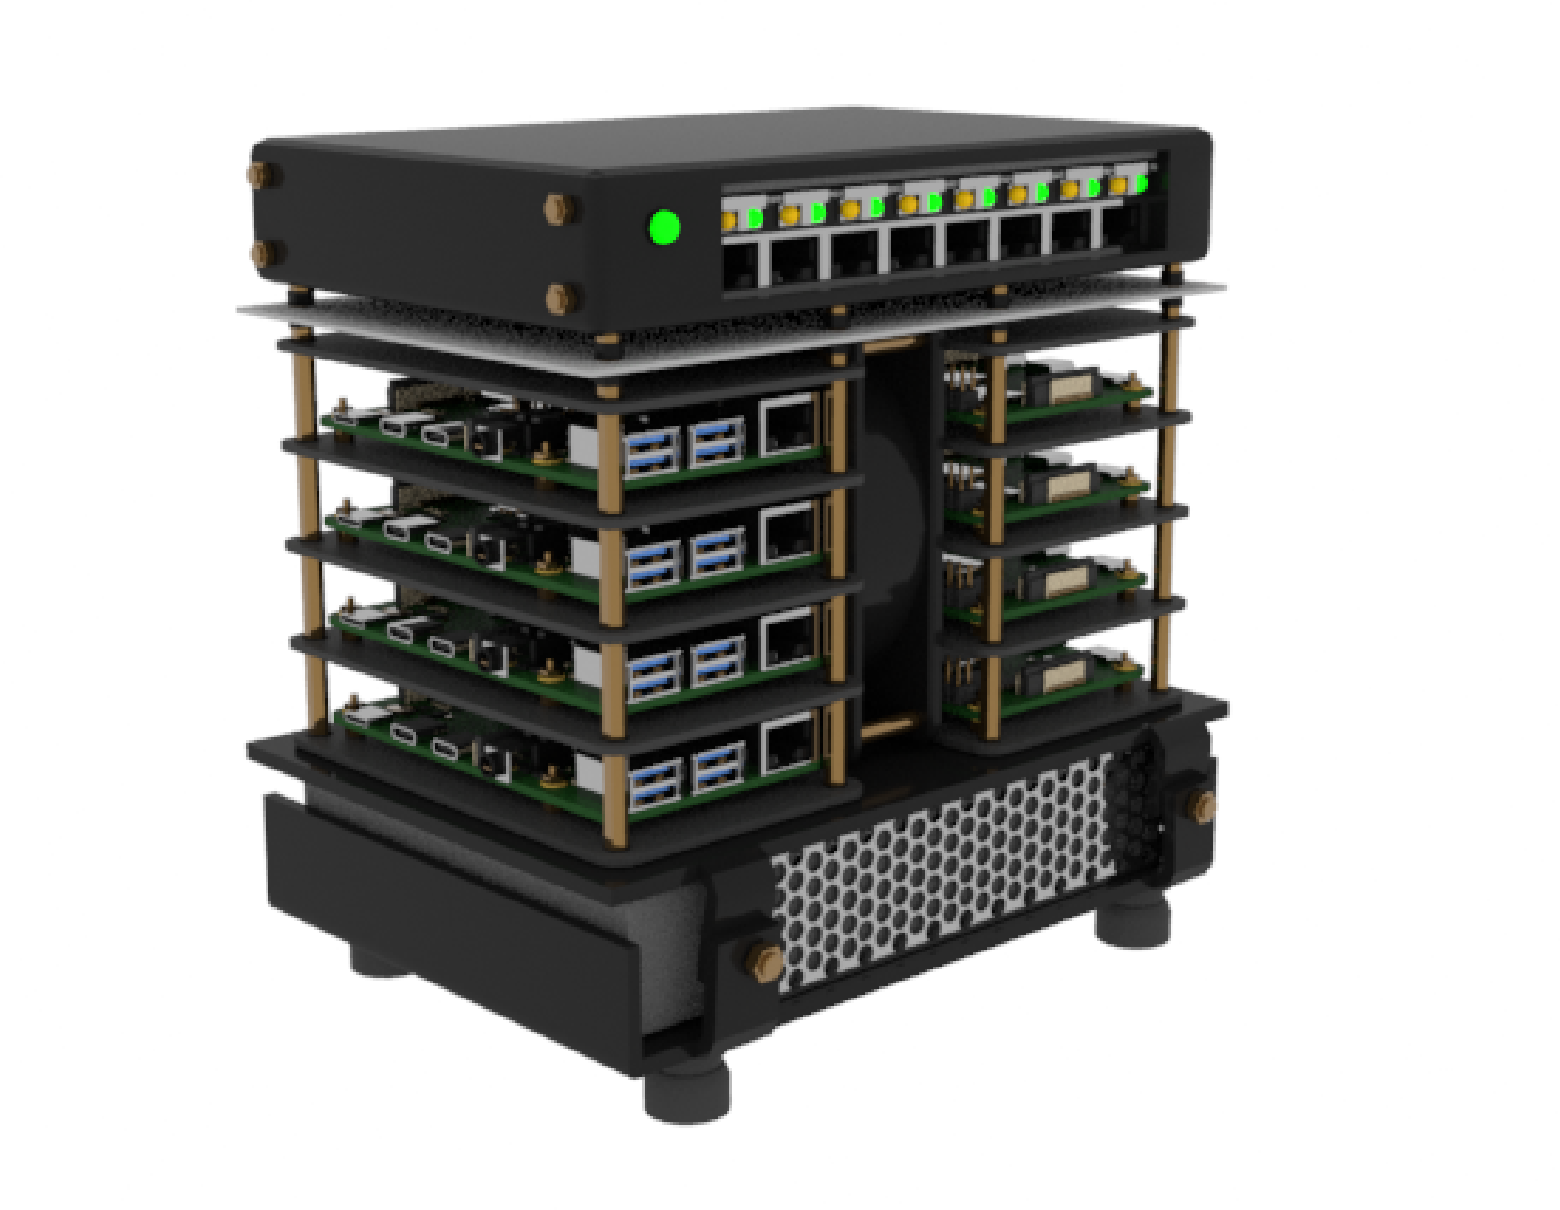
\includegraphics[width=\textwidth]{img/render_cluster_1_provisional.png}
  \caption{Render frontal del cluster}
  \label{fig:render_cluster_1}
\end{figure}

\section{Infraestructura Software}
\label{sec:infra_software}

\subsection{Requisitos funcionales}

\subsection{Requisitos no funcionales}
